\documentclass[aspectratio=169,11pt]{beamer}

\usepackage[brazilian]{babel}
\usepackage[utf8]{inputenc}
\usepackage[T1]{fontenc}
\usepackage{amsmath,amssymb,amsfonts,mathtools}
\usepackage{booktabs}
\usepackage{listings}
\usepackage{xcolor}

\usepackage{graphicx}

\setbeamertemplate{navigation symbols}{}
\setbeamertemplate{headline}{}
\setbeamertemplate{footline}{}
\usebackgroundtemplate{%
    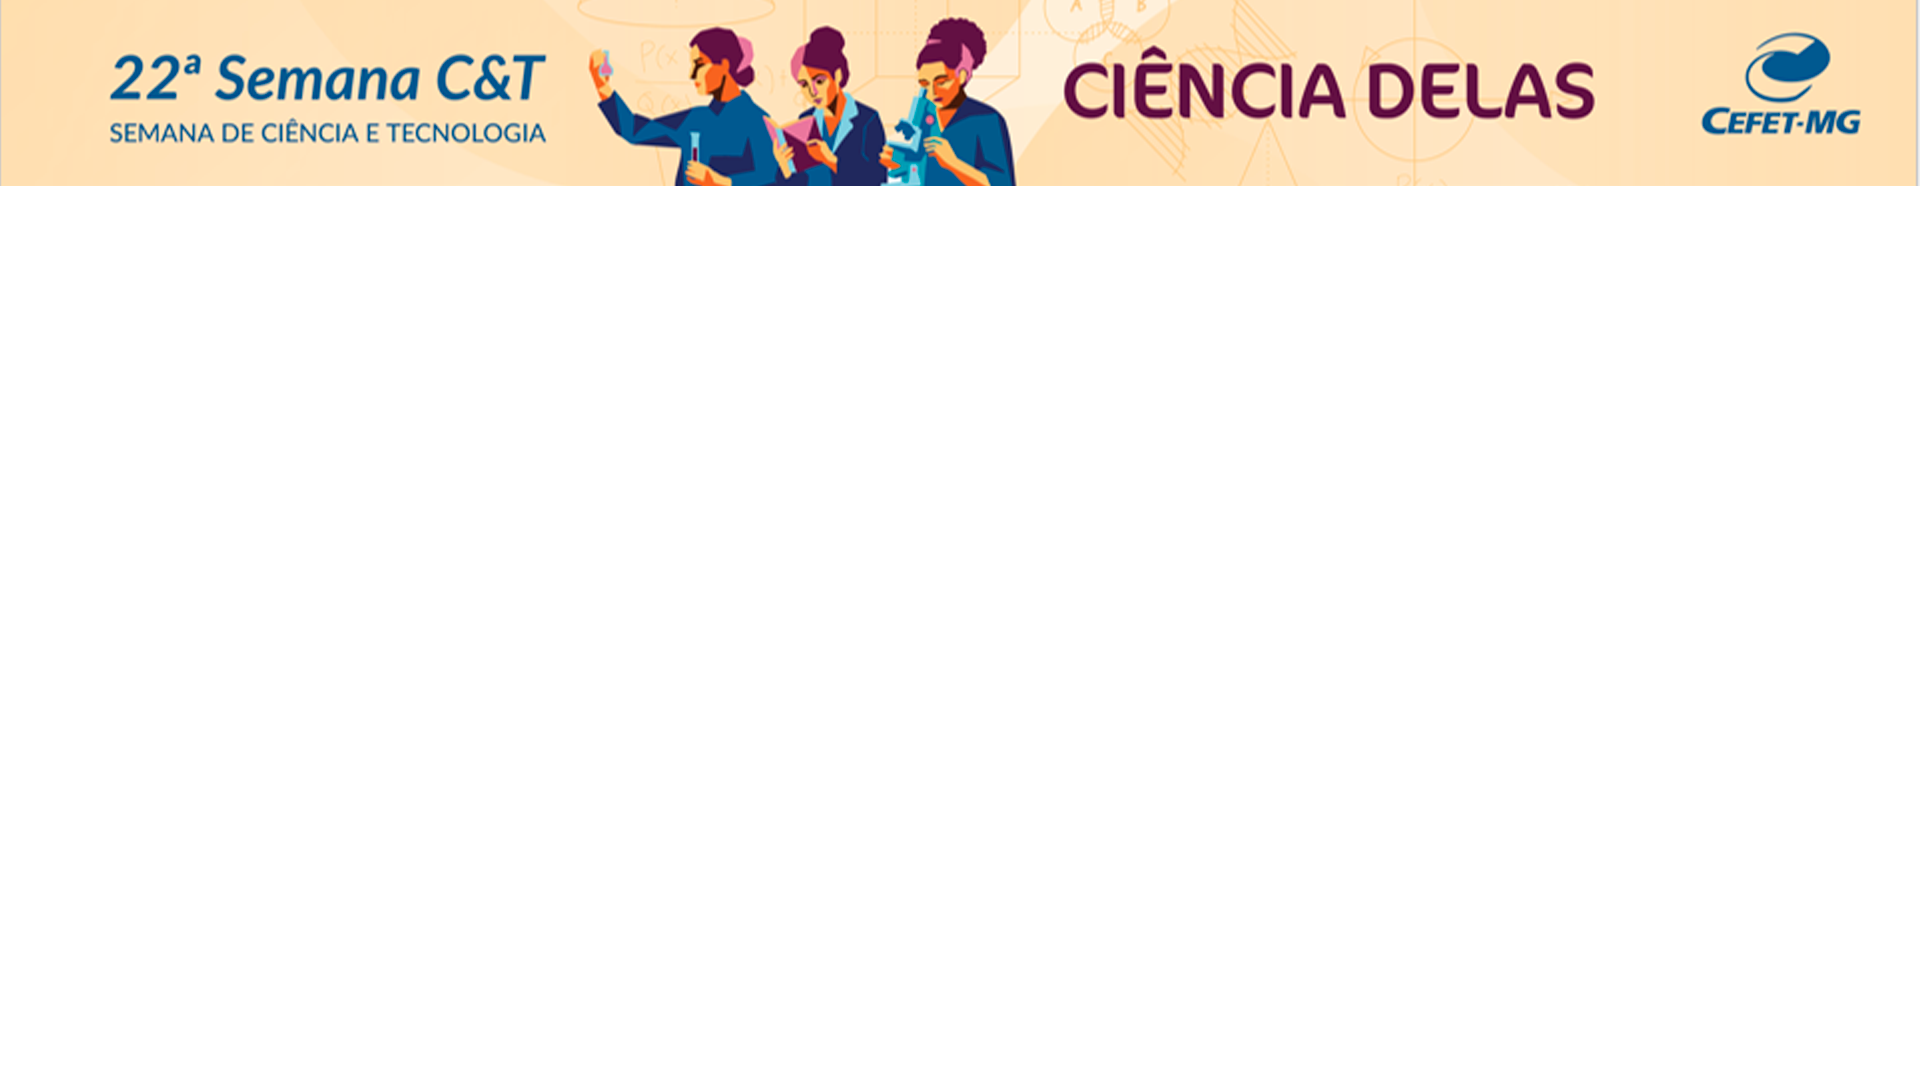
\includegraphics[
        width=\paperwidth,
        height=\paperheight-1cm
    ]{capacy.png}%
}

\setbeamersize{
    text margin left=1.0cm,
    text margin right=1.0cm
}

\setbeamerfont{frametitle}{
    size=\Large,
    series=\bfseries
}

\setbeamercolor{frametitle}{
    fg=black
}

\setbeamertemplate{frametitle}{%
    \vspace{1.35cm}
    \insertframetitle
    \vspace{0.15cm}
}


\usetheme{Madrid}
\setbeamertemplate{navigation symbols}{}

\lstset{
  basicstyle=\ttfamily\small,
  columns=fullflexible,
  keepspaces=true,
  showstringspaces=false,
  frame=single,
  breaklines=true
}

\title[Programação Funcional]{Programação Funcional:\\do Cálculo Lambda à Implementação de Métodos Numéricos}
\author[Ribas et al.]{Enzo Rocha Leite Diniz Ribas \and Luis A. D'Afonseca \and Lucas Martins Rocha}
\institute[CEFET-MG]{Centro Federal de Educação Tecnológica de Minas Gerais\\Belo Horizonte -- MG}
\date{22ª Semana de Ciência \& Tecnologia do CEFET-MG}

\begin{document}

\begin{frame}
  \titlepage
\end{frame}

\begin{frame}{Objetivo da apresentação}
  \begin{block}{Pergunta central}
    Como ideias de programação funcional ajudam a escrever, testar e raciocinar sobre métodos numéricos?
  \end{block}

  \vspace{0.2cm}
  \begin{enumerate}
    \item Funções matemáticas e funções em programas.
    \item Cálculo lambda como modelo formal de aplicação de funções.
    \item Composição, erros explícitos e iteração numérica.
    \item Newton--Raphson como exemplo principal.
  \end{enumerate}

  \vspace{0.2cm}
\end{frame}

\section{Motivação}

\begin{frame}{Da função matemática ao programa}
  Na matemática, uma função associa entradas válidas a saídas:
  \begin{equation}\label{eq:raiz-dominio}
    f:\mathbb{R}\longrightarrow \mathbb{R},\qquad
    f(x)=\sqrt{x}.
  \end{equation}

  \begin{center}
    \begin{tabular}{c|c}
      \toprule
      Entrada & Resultado em $\mathbb{R}$ \\
      \midrule
      $4$ & $2$ \\
      $0$ & $0$ \\
      $-1$ & não definido em $\mathbb{R}$ \\
      \bottomrule
    \end{tabular}
  \end{center}

  \begin{alertblock}{Problema computacional}
    Como o programa deve representar uma entrada fora do domínio?
  \end{alertblock}
\end{frame}

\begin{frame}[fragile]{Imperativo: erro fora da assinatura}
  \begin{lstlisting}[language=Java]
double sqrt(double x) {
    if (x < 0)
        throw new IllegalArgumentException();
    return Math.sqrt(x);
}
  \end{lstlisting}

  \begin{itemize}
    \item A assinatura sugere apenas: \texttt{double -> double}.
    \item A exceção existe, mas aparece fora do fluxo normal do valor.
    \item O chamador precisa conhecer esse comportamento por documentação, teste ou leitura do código.
  \end{itemize}

  \begin{block}{Ideia funcional}
    Tornar o caso inválido parte explícita do resultado.
  \end{block}
\end{frame}

\begin{frame}{Funcional: erro como valor}
  Em vez de esconder a falha em uma exceção, podemos modelar:
  \begin{equation*}
    \texttt{safeSqrt}:\mathbb{R}\longrightarrow \texttt{Maybe}\;\mathbb{R}.
  \end{equation*}

  \begin{equation*}
    \texttt{safeSqrt}(x)=
    \begin{cases}
      \texttt{Just}(\sqrt{x}), & x\geq 0,\\
      \texttt{Nothing}, & x<0.
    \end{cases}
  \end{equation*}

  \begin{center}
    \begin{tabular}{c|c}
      \toprule
      Entrada & Resultado \\
      \midrule
      $4$ & \texttt{Just 2} \\
      $0$ & \texttt{Just 0} \\
      $-1$ & \texttt{Nothing} \\
      \bottomrule
    \end{tabular}
  \end{center}
\end{frame}

\section{Cálculo Lambda}

\begin{frame}{Cálculo lambda: três ideias}
  O cálculo lambda é um modelo formal para representar funções e computações.

  \begin{center}
    \begin{tabular}{c|c|c}
      \toprule
      Ideia & Forma & Leitura \\
      \midrule
      Abstração & $\lambda x.\;e$ & função que recebe $x$ e calcula $e$ \\
      Aplicação & $e_1\;e_2$ & aplica $e_1$ ao argumento $e_2$ \\
      Redução & $(\lambda x.\;e)\;v \to e[x:=v]$ & substitui $x$ por $v$ em $e$ \\
      \bottomrule
    \end{tabular}
  \end{center}

  \vspace{0.2cm}
  Exemplo:
  \begin{equation*}
    \lambda x.\;x^2
  \end{equation*}
  representa a função que recebe $x$ e devolve $x^2$.
\end{frame}

\begin{frame}{Beta Reduction}
  Considere a função que soma $1$ ao argumento:
  \begin{equation*}
    (\lambda x.\;x+1)\;4.
  \end{equation*}

  A aplicação é avaliada por substituição:
  \begin{equation*}
    (\lambda x.\;x+1)\;4
    \longrightarrow
    4+1
    \longrightarrow
    5.
  \end{equation*}

  Outro exemplo, com função quadrática:
  \begin{equation*}
    (\lambda x.\;x\cdot x + 1)\;3
    \longrightarrow
    3\cdot 3+1
    \longrightarrow
    10.
  \end{equation*}

  \begin{block}{No contexto de métodos numéricos}
    Uma iteração numérica também aplica uma transformação a uma aproximação atual para produzir a próxima.
  \end{block}
\end{frame}

\begin{frame}{Funções de Alta Ordem (Funções que recebem e retornam funções)}
  Em cálculo lambda, funções podem ser argumentos de outras funções.

  \begin{equation*}
    \operatorname{aplicarDuasVezes}=\lambda g.\lambda x.\;g(g(x)).
  \end{equation*}

  Se $g(x)=x+1$:
  \begin{equation*}
    (\lambda \textcolor{blue}{g}.\lambda \textcolor{red}{x}.\;\textcolor{blue}{g}(\textcolor{blue}{g}(\textcolor{red}{x})))\;\textcolor{blue}{(\lambda y.\;y+1)}\;\textcolor{red}{3}
    \longrightarrow
    5.
  \end{equation*}

  \begin{block}{Ideia importante}
    Métodos iterativos seguem exatamente essa estrutura: aplicar repetidamente uma função de atualização.
  \end{block}
\end{frame}

\begin{frame}{Currying e especialização}
  Uma função de dois argumentos pode ser vista como uma função que retorna outra função:
  \begin{equation*}
    f(x,y)=x+y
    \qquad\Longleftrightarrow\qquad
    f=\lambda x.\lambda y.\;x+y.
  \end{equation*}

  Fixando $x=10$:
  \begin{equation*}
    \operatorname{somar10}=f(10)=\lambda y.\;10+y.
  \end{equation*}

  Logo:
  \begin{equation*}
    \operatorname{somar10}(5)=15.
  \end{equation*}

  \begin{block}{Uso prático}
    Currying permite criar funções especializadas a partir de funções gerais.
  \end{block}
\end{frame}

\begin{frame}{Composição com contexto}
  Algumas operações possuem restrições de domínio:
  \begin{equation*}
    x \xrightarrow{\sqrt{\phantom{x}}} \sqrt{x}
      \xrightarrow{\log} \log(\sqrt{x}).
  \end{equation*}

  Usando \texttt{Maybe}, cada etapa informa se produziu valor ou falhou:
  \begin{equation*}
    \texttt{Maybe}\;A
    \longrightarrow
    (A\rightarrow\texttt{Maybe}\;B)
    \longrightarrow
    \texttt{Maybe}\;B.
  \end{equation*}

  \begin{center}
    \begin{tabular}{c|c}
      \toprule
      Entrada & Resultado de $\log(\sqrt{x})$ \\
      \midrule
      $4$ & $\texttt{Just}(\log 2)$ \\
      $0$ & \texttt{Nothing}, pois $\log(0)$ é inválido \\
      $-1$ & \texttt{Nothing}, pois $\sqrt{-1}$ é inválido \\
      \bottomrule
    \end{tabular}
  \end{center}
\end{frame}

\section{Programação Funcional}

\begin{frame}{O que é programação funcional?}
  A programação funcional trata \textbf{funções como abstrações centrais da computação}.

  \vspace{0.25cm}
  Em vez de organizar o programa principalmente por comandos e mutações de estado,
  ela organiza a computação por \textbf{transformações de dados}.

  \vspace{0.3cm}
  \begin{columns}[T]
    \column{0.48\textwidth}
    \begin{itemize}
      \item funções de primeira classe;
      \item funções puras;
      \item imutabilidade.
    \end{itemize}

    \column{0.48\textwidth}
    \begin{itemize}
      \item composição;
      \item recursão;
      \item efeitos controlados.
    \end{itemize}
  \end{columns}
\end{frame}

\begin{frame}{Funções de primeira classe}
  Uma função é de primeira classe quando pode ser tratada como um valor.

  \vspace{0.2cm}
  Isso significa que ela pode ser:

  \begin{itemize}
    \item armazenada em uma variável;
    \item passada como argumento;
    \item retornada por outra função.
  \end{itemize}

  \begin{exampleblock}{Ligação com métodos numéricos}
    Um método de Newton genérico recebe $f$ e $f'$ como argumentos.
  \end{exampleblock}

  \begin{equation*}
    \texttt{newtonStep}(f,f',x)
    =
    x-\frac{f(x)}{f'(x)}.
  \end{equation*}
\end{frame}

\begin{frame}{Funções puras}
  Uma função pura depende apenas dos argumentos de entrada.

  \begin{block}{Definição prática}
    Para a mesma entrada, produz sempre a mesma saída e não altera o estado observável do programa.
  \end{block}

  \begin{equation}\label{eq:funcao-pura}
    f:\mathbb{R}\longrightarrow\mathbb{R},
    \qquad
    f(x)=x^2+1.
  \end{equation}

  \vspace{0.15cm}
  A chamada da função pode ser entendida como uma transformação matemática:

  \begin{equation*}
    x\xmapsto{\ f\ }f(x).
  \end{equation*}
\end{frame}

\begin{frame}[fragile]{Efeito colateral}
  \textbf{Com efeito colateral:}

  \begin{lstlisting}
int counter = 0;

int f(int x) {
    counter++;
    return x * x;
}
  \end{lstlisting}

  \begin{alertblock}{O que acontece?}
    Além de retornar $x^2$, a função altera \texttt{counter}. Portanto,
    seu comportamento não é descrito apenas por $x\mapsto x^2$.
  \end{alertblock}
\end{frame}

\begin{frame}[fragile]{Função pura}
  \textbf{Sem efeito colateral:}

  \begin{lstlisting}
int f(int x) {
    return x * x;
}
  \end{lstlisting}

  \begin{equation*}
    f:x\longmapsto x^2.
  \end{equation*}

  \begin{block}{Consequência}
    A função fica mais fácil de testar, compor e reproduzir.
  \end{block}
\end{frame}

\begin{frame}{Imutabilidade}
  Imutabilidade significa evitar sobrescrever valores já criados.

  \vspace{0.2cm}
  Em um método iterativo, isso combina bem com a própria notação matemática:

  \begin{equation*}
    x_0\longrightarrow x_1\longrightarrow x_2\longrightarrow\cdots
  \end{equation*}

  \vspace{0.2cm}
  Cada aproximação é um novo valor, não a ``mesma variável'' modificada.

  \begin{exampleblock}{Leitura numérica}
    Em vez de pensar apenas em \texttt{x = ...}, pensamos em uma sequência
    $x_0,x_1,x_2,\ldots$.
  \end{exampleblock}
\end{frame}

\begin{frame}{Composição}
  Composição é construir uma função a partir de outras funções.

  \begin{equation}\label{eq:composicao}
    f:A\longrightarrow B,
    \qquad
    g:B\longrightarrow C
    \qquad\Rightarrow\qquad
    g\circ f:A\longrightarrow C.
  \end{equation}

  \vspace{0.15cm}
  A aplicação composta é:

  \begin{equation*}
    (g\circ f)(x)=g(f(x)).
  \end{equation*}

  \begin{block}{Em métodos numéricos}
    Podemos separar cálculo do passo, validação, critério de parada e atualização.
  \end{block}
\end{frame}

\begin{frame}{Recursão}
  Recursão descreve uma computação em termos dela mesma.

  \vspace{0.15cm}
  Um exemplo clássico é o fatorial:

  \begin{equation*}
    n! =
    \begin{cases}
      1, & n=0,\\
      n\cdot(n-1)!, & n>0.
    \end{cases}
  \end{equation*}

  \begin{exampleblock}{Ligação com iteração}
    Métodos numéricos também podem ser vistos recursivamente:
  \end{exampleblock}

  \begin{equation*}
    x_{n+1}=N(x_n).
  \end{equation*}
\end{frame}

\begin{frame}{Efeitos controlados}
  Nem toda computação é uma função matemática pura.

  \vspace{0.2cm}
  Programas reais lidam com:

  \begin{itemize}
    \item erros;
    \item entrada e saída;
    \item estado;
    \item valores ausentes;
    \item falhas de convergência.
  \end{itemize}

  \begin{block}{Ideia funcional}
    O efeito não precisa ficar escondido. Ele pode aparecer no tipo ou no resultado.
  \end{block}
\end{frame}

\begin{frame}{Efeitos controlados em métodos numéricos}
  Em Newton--Raphson, nem toda execução converge.

  \vspace{0.2cm}
  Em vez de retornar apenas um número, o algoritmo pode retornar um resultado estruturado:

  \begin{equation*}
    \texttt{NewtonResult}
    =
    \texttt{Converged}
    \mid
    \texttt{MaxIterations}
    \mid
    \texttt{InvalidDerivative}
    \mid\cdots
  \end{equation*}

  \begin{alertblock}{Ponto central}
    A falha deixa de ser um comportamento escondido e passa a fazer parte da interface do método.
  \end{alertblock}
\end{frame}

\begin{frame}{Ponte com métodos numéricos}
  Considere a função de atualização de Newton:

  \begin{equation}\label{eq:newton-pf}
    N_{f,f'}(x)
    =
    x-\frac{f(x)}{f'(x)}.
  \end{equation}

  A iteração é a aplicação repetida dessa função:

  \begin{equation}\label{eq:iteracao-newton-pf}
    x_{n+1}=N_{f,f'}(x_n).
  \end{equation}

  \begin{center}
    \small
    funções de primeira classe $\rightarrow$ função pura $\rightarrow$ composição $\rightarrow$ iteração
  \end{center}
\end{frame}

\section{Métodos Numéricos}

\begin{frame}{Métodos numéricos como transformações}
  Métodos numéricos são algoritmos construídos a partir de transformações matemáticas.

  Para Newton--Raphson:
  \begin{equation}\label{eq:newton-raphson}
    x_{n+1}=x_n-\frac{f(x_n)}{f'(x_n)}.
  \end{equation}

  Definindo a função de atualização:
  \begin{equation}\label{eq:funcao-atualizacao-newton}
    N_f(x)=x-\frac{f(x)}{f'(x)},
  \end{equation}

  a sequência de aproximações é:
  \begin{equation*}
    x_0,\quad N_f(x_0),\quad N_f(N_f(x_0)),\quad N_f^3(x_0),\ldots
  \end{equation*}

  \begin{block}{Perspectiva funcional}
    A iteração é aplicação repetida de uma função.
  \end{block}
\end{frame}

\begin{frame}{Exemplo numérico: raiz de $x^2-2$}
  Queremos aproximar $\sqrt{2}$ resolvendo:
  \begin{equation*}
    f(x)=x^2-2,\qquad f'(x)=2x.
  \end{equation*}

  A função de Newton é:
  \begin{equation*}
    N_f(x)=x-\frac{x^2-2}{2x}=\frac{x}{2}+\frac{1}{x}.
  \end{equation*}

  Começando com $x_0=1$:
  \begin{center}
    \begin{tabular}{c|c}
      \toprule
      Iteração & Aproximação \\
      \midrule
      $x_0$ & $1.0000$ \\
      $x_1=N_f(x_0)$ & $1.5000$ \\
      $x_2=N_f(x_1)$ & $1.4167$ \\
      $x_3=N_f(x_2)$ & $1.4142$ \\
      \bottomrule
    \end{tabular}
  \end{center}
\end{frame}

\begin{frame}[fragile]{Newton: implementação funcional}
  Um passo de Newton pode ser escrito como uma função pura:

  \begin{lstlisting}[language=Haskell]
newtonStep f df x = x - f x / df x
  \end{lstlisting}

  Para $f(x)=x^2-2$:

  \begin{lstlisting}[language=Haskell]
f  x = x*x - 2
df x = 2*x

x1 = newtonStep f df x0
  \end{lstlisting}

  \begin{block}{Leitura matemática}
    \texttt{newtonStep} recebe $f$, $f'$ e $x_n$, devolvendo $x_{n+1}$.
  \end{block}
\end{frame}

\begin{frame}{Falhas também fazem parte do método}
  Newton--Raphson pode falhar por razões matemáticas ou computacionais:

  \begin{columns}
    \column{0.5\textwidth}
    \begin{itemize}
      \item derivada nula;
      \item domínio inválido;
      \item divergência;
    \end{itemize}

    \column{0.5\textwidth}
    \begin{itemize}
      \item máximo de iterações;
      \item tolerância não atingida;
      \item perda de precisão.
    \end{itemize}
  \end{columns}

  \vspace{0.25cm}
  Uma saída mais informativa é:
  \begin{equation*}
    \texttt{NewtonResult}=\texttt{Converged}\mid\texttt{MaxIterations}\mid\texttt{InvalidDerivative}\mid\cdots
  \end{equation*}

  \begin{alertblock}{Ponto central}
    O algoritmo não precisa fingir que todo resultado é apenas um número.
  \end{alertblock}
\end{frame}

\section{Fechamento}

\begin{frame}{Síntese}
  \begin{enumerate}
    \item Funções puras aproximam o programa da notação matemática.
    \item Cálculo lambda formaliza abstração, aplicação e substituição.
    \item Currying e funções de alta ordem permitem especialização.
    \item Contextos como \texttt{Maybe} tornam falhas explícitas.
    \item Métodos numéricos podem ser mais naturalmente modelados como composição e aplicação repetida de funções.
  \end{enumerate}

  \vspace{0.2cm}
  \begin{block}{Mensagem final}
    A programação funcional não substitui a imperativa, mas oferece ferramentas para estruturar problemas matemáticos de forma mais natural e segura.
  \end{block}
\end{frame}

\begin{frame}{Contato}
    \begin{center}
        \Large\textbf{Enzo Rocha Leite Diniz Ribas}
    \end{center}
    
    \vspace{0.2cm}
    \begin{columns}[T]
        \column{0.5\textwidth}
        \begin{itemize}
        \item GitHub: \texttt{@oenzoribas}
        \item LinkedIn: \texttt{Enzo Ribas}
        \item E-mail: \texttt{enzorochaleitedinizribas@gmail.com}
        \item Instagram: \texttt{ribas\_enzo}
        \end{itemize}
    \end{columns}
\end{frame}

\begin{frame}{Agradecimentos}
  \begin{center}
    \Huge\textbf{Do Cálculo Lambda à Programação Funcional.}
  \end{center}

  \vfill
  \begin{center}
    \normalsize Thanks for your attention.
  \end{center}
\end{frame}

\begin{frame}{Referências}

  \scriptsize

  \begin{columns}[T,onlytextwidth]

    % =========================
    % COLUNA ESQUERDA
    % =========================
    \column{0.49\textwidth}

    \begin{thebibliography}{9}

      \bibitem{pierce}
      PIERCE, B. C.
      \newblock \emph{Types and Programming Languages}.
      \newblock MIT Press, 2002.

      \bibitem{hutton}
      HUTTON, G.
      \newblock \emph{Programming in Haskell}.
      \newblock Cambridge University Press.

      \bibitem{Chapra}
      CHAPRA, S. C.; CANALE, R. P.
      \newblock \emph{Numerical Methods for Engineers}.
      \newblock McGraw-Hill Education.

    \end{thebibliography}

    % =========================
    % COLUNA DIREITA
    % =========================
    \column{0.49\textwidth}

    \begin{thebibliography}{9}

      \setcounter{enumiv}{3}

      \bibitem{Church}
      CHURCH, A.
      \newblock \emph{An Unsolvable Problem of Elementary Number Theory}.
      \newblock American Journal of Mathematics, 1936.

      \bibitem{burden}
      BURDEN, R. L.; FAIRES, J. D.
      \newblock \emph{Numerical Analysis}.
      \newblock Cengage Learning.

    \end{thebibliography}

  \end{columns}

\end{frame}
\end{document}
